%%%%%%%%%%%%%%%%%%%%%%%%%%%%%%%%%%%%%%%%%%%%%%%%%%%%%%%%%%%%%%%%%%%%%%
%
\section{Congestion level at different timestamps} %Befehlt section steht für kapitel
%
%%%%%%%%%%%%%%%%%%%%%%%%%%%%%%%%%%%%%%%%%%%%%%%%%%%%%%%%%%%%%%%%%%%%%%

\subsection{untertitel}
\subsubsection{unteruntertitel}
\paragraph{unnötiger paragraph}

Beispiel Text:

Hier kann man sehen, wie dann der Text stehen wird. In Latex schreibt man normalerweise nie \textbf{fett}, sondern wenn etwas hervorgehoben werden soll, benutzt man den befehl \emph{emph}, welcher für emphazise steht.

Eine weitere Besonderheit sind aufzählungen:
\begin{itemize}
    \item der erste punkt
    \item der zweite punkt
\end{itemize}


Bei aufuählungen wird immer erst das kommando gegebne, dass nun aufgezählt wird mittels \emph{itemize} und dann jeder punkt wird zuvor als \emph{item} definiert. 

Bei numerierungen, also erstens zweiten etc., geht man genau gleich vor, allerdings mit dem kommando \emph{begin enumerate}

\begin{enumerate}
    \item erste zahl
    \item zweite zahl
    \item dritte zahl
    \begin{enumerate}
        \item noch eine stufe weiter
    \end{enumerate}
    \item und noch eine zum Abschluss
\end{enumerate}

Wie man sehen kann, kann man mitten in der aufzählung oder nummerierung einfach noch eine ebene weiter rein gehen, indem man nochmals den begin befehl gibt. Latex macht dabei selber die korrekte nummerierung weiter:)

Gewisse Zeichen sind für latex schon vorreserviert - latex liest sie als befehl auch wenn sie nicht als solcher gedacht sind. Dazu gehört der backslash und das \dq und\dq{} zeichen. dieses wird einfach mit einem backslash erst versehen und so als command ausgeführt \&. Im code seht ihr auch, dass die Anführungszeichen etwas umständlich geschrieben wurden... aber die braucht man ja auch nicht so oft. Letzten endes sind es vlt so 10 befehle die man immer wieder braucht und sich lohnen zu merken, alles andere kann man einfach googeln. Die online community ist fast noch besser als bei R


\createfigure% Befehl, dass eine figur eingeführt wird, welche dann auch im abbildungsverzeichnis erscheint
[] % wo soll die Datei sein (leer = Latex sucht für dich, h = mehr oder weniger hier (latex sucht soweit es geht), H = genau hier - führt unter umständen zu viel weissem platz
{Titel der Figur im Abb. Verzeichnis}% Die Beschriftung wie sie im abb. verzeichnis sein soll
{Titel über der Figur}% ¨titel der grafik gleich darüber
{\label{fig:michi}}% das label, welches für querverweise verwendet wird
{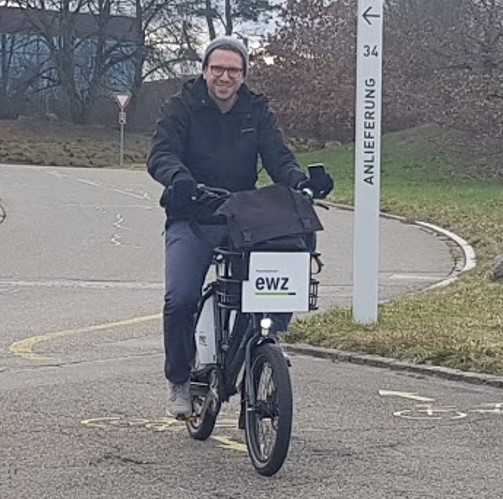
\includegraphics[width=1.0\textwidth, angle=0]{figures/Bild1.jpg}}% der eigentliche pfad mit allenfalls nötigem angle um das bild zu drehen (in grad)
{eigener schnappschuss} % die quelle (das wort quelle wird automatisch generiert)

Im code seht ihr, wie das bild eingefügt wurde. Das ist hier vom IVT so \emph{sophisticated} gemacht worden. Für latex würde eine kurze zeile reichen. Es ist dennoch sehr praktisch und mankann alles sowieso immer copypasten. So kann ich jetzt einfach auf die \cref{fig:michi} querverweisen.

Was nicht ganz so trivial ist, aber wenn mans mal drin hat super nützlich ist, ist das zitieren und einfügen von quellen. Hier mal als Beispie \citep{AxhausenEtAl_2002} oder ohne klammern \cite{AxhausenEtAl_2002}. Das codewort entnimmt man der bibliothek, welche auch hier im file ist unter \_latexfiles/bibs/all-ger.bib (habe gerade festgestellt, dass nur my.bib auf overleaf funktioniert.
Dort sind schon viele für das IVT wichtige drin abgespeichert, die man einfach kopieren kann. Wenn man was von google scholar nimmt, kann man dort auch einfach kopieren. 
Macht man jedoch einen ganz neuen eintrag wie zum beispiel vom velohandbuch, so kommt ein bisschen trial\&error zum zug... ich kann die sonst dann machen. Das braucht ein wenig übung, und selbst dann kann man durchdrehen. 

Das mühsahmste, im vergleich zu office, sind tabellen in latex. Ich kann das dann mal zeigen, wenn es soweit ist. sie sehen jedoch auch viel schöner aus am schluss:)

\cite{axhausen1909histologischen}